\chapter{The Propagation of Radio Waves}\labch{propagation}

The study of radio wave propagation establishes a connection between the theoretical foundation of electromagnetic theory and the practical implementation of wireless communication systems. In order to construct sophisticated algorithms for ray tracing and channel modeling (topics that will be addressed in the subsequent chapters of this book), it is essential to first understand the fundamental physics governing the transmission of energy from a source to a destination. This chapter serves as a short introduction to the fundamental concepts required to understand the propagation of radio waves, rigorously deriving their behavior as they traverse \gls{free space}, interact with material boundaries, and navigate complex environments. In the next sections, we assume that the reader is familiar with vector analysis and basic electromagnetic theory. For a more in-depth introduction to electromagnetic theory, including the necessary background in vector analysis, we recommend reading Griffiths's \emph{Introduction to Electrodynamics}~\sidecite{Griffiths2024}, as well as Saunders and Aragón-Zavala's \emph{Antennas and Propagation for Wireless Communication Systems}~\sidecite{Saunders2024} for more applied content on radio propagation. Moreover, the present chapter takes great inspiration from both of these textbooks, and we will often refer to them for further reading.

The foundation of ray tracing is based on two pillars: the concept of a radio channel and classical electrodynamics, mathematically described by Maxwell's equations. We first define what we mean by a radio channel. Then, starting from Maxwell's equations, we derive the wave equation to elucidate the oscillatory nature of electromagnetic fields. From there, we examine the behavior of plane waves, including their polarization and propagation through lossy media. We then explore how these waves interact with material boundaries through reflection and refraction, governed by Snell's law and Fresnel's equations, as well as other effects such as diffraction and scattering. Finally, we introduce the fundamentals of antennas, which serve as the sources and sinks of these radio waves, and establish the basic link budget equation for \gls{line-of-sight} communication.

\section{Fundamentals of the Wireless Channel}

The wireless channel is the physical medium that connects the transmitter and receiver, and understanding its characteristics is crucial for the design and analysis of any wireless communication system. Whether for cellular networks, satellite links, or local area networks, the channel imposes fundamental limits on performance.

A generic communication system can be described by the architecture proposed by Claude Shannon~\sidecite{Shannon1948}, usually depicted as consisting of five functional blocks: the information source, the transmitter, the channel, the receiver, and the destination (see \reffig{generic_system}). The transmitter processes the information into a signal suitable for the channel, while the receiver's task is to recover this information from the received signal, which has been degraded by the channel.

\begin{figure*}
  \centering
  \caption{Simplified schematic of a generic communication system where a podcaster broadcasts a show to a listener's smartphone through a wireless channel, inspired by~\cite[Fig.~1]{Shannon1948} and~\cite[Fig.~1.2]{Saunders2024}.}
  \inputtikz{channel}
  \labfig{generic_system}
\end{figure*}

The degradation caused by the channel can be mathematically modeled as a linear time-varying filter. The received signal $y(t)$ is generally expressed as the convolution of the transmitted signal $x(t)$ with the channel's impulse response $h(t)$, corrupted by additive noise $n(t)$,
\begin{equation}
  y(t) = h(t) \ast x(t) + n(t).
\end{equation}

This formulation clearly distinguishes between two main types of impairments: additive noise and multiplicative fading effects.

\subsection{Additive Noise}

The term $n(t)$ represents additive noise, which generally arises from thermal fluctuations within the receiver electronics or from external interference sources such as cosmic radiation and man-made signals. In many theoretical analyses, this noise is modeled as a Gaussian random process. While noise sets a strict lower bound on the detectable signal level, in many practical wireless scenarios---particularly in dense urban settings---system performance is constrained primarily by the complex multiplicative effects of the channel rather than simple additive noise.

\subsection{Multiplicative Effects}

The impulse response $h(t)$ encapsulates the multiplicative effects resulting from the complex propagation environment. As the radio wave travels from the transmitter to the receiver, it interacts with physical objects through several mechanisms:
\begin{itemize}
  \item \emph{Reflection} from large, smooth surfaces such as building facades or the ground.
  \item \emph{Transmission and absorption} as the wave passes through materials like glass, brick, or foliage, losing energy in the process.
  \item \emph{Diffraction} around sharp edges like building corners or rooflines, allowing signals to reach shadowed areas.
  \item \emph{Scattering} from rough surfaces or objects that are small relative to the \gls{wavelength}.
\end{itemize}

These interactions cause the signal to arrive at the receiver via multiple paths, leading to constructive and destructive interference known as fading. These variations occur over different spatial scales, as illustrated in \reffig{fading_scales}.

\begin{figure*}
  \centering
  \inputtikz{three-scales}
  \caption{The three scales of signal variation, adapted from~\cite[Fig.~1.5]{Saunders2024}.}
  \labfig{fading_scales}
\end{figure*}

\begin{itemize}
  \item \emph{Path loss} is the deterministic decay of average signal power as the distance between transmitter and receiver increases. It represents the large-scale trend influenced by the geometry of the environment and \glshyph{free space} spreading.
  \item \emph{Shadowing} represents medium-scale variations caused by specific obstacles blocking the direct path, such as buildings or hills. Shadowing is often modeled as a log-normal random process superimposed on the path loss~\sidecite[][Chap.~9]{Saunders2024}.
  \item \emph{Fast fading} consists of the small-scale, rapid fluctuations in signal amplitude and phase occurring over distances of just a few \glspl{wavelength}. This results from the vector addition of multiple signal copies arriving at the receiver with different phases.
\end{itemize}

The next chapters will present how ray tracing can be used to model these multiplicative effects by simulating the physical interactions of rays with the environment, providing a powerful tool for predicting channel behavior in complex scenarios.

\subsection{The Electromagnetic Spectrum}

The electromagnetic spectrum is a fundamental resource for wireless transmissions. Commercial and military radio systems typically operate within the frequency range of \qty{3}{\kilo\hertz} to \qty{300}{\giga\hertz}. The choice of operating frequency involves several trade-offs. For example, higher frequency bands provide larger available bandwidths for high-speed data transmission, but this comes at the cost of increased path loss and weaker penetration capabilities through building materials. As a rule of thumb, the \glshyph{free space} path loss formula predicts that signal power decreases with the square of both frequency and distance. \reffig{frequency_bands} and \reftab{frequency_bands} provide a summary of the standard frequency bands used in wireless communications~\sidecite[-.7cm]{ITU-R-V.431}.

\begin{figure*}
  \centering
  \inputtikz{radio-spectrum}
  \caption{Frequency spectrum used in wireless communications, adapted from~\cite[Fig.~1.6]{Saunders2024}.}
  \labfig{frequency_bands}
\end{figure*}

\begin{table*}
  \caption{Naming conventions for frequency bands, reproduced from~\cite[Table~1.1]{Saunders2024}.}
  \labtab{frequency_bands}
  \centering
  \sisetup{range-units=single,range-phrase=\,--\,}
  \begin{tabular}{@{}lr c lr@{}}
    \toprule
    & Frequency & & & Frequency \\
    Band name & range & \hspace{.3cm} & Band name & range \\
    \cmidrule{1-2} \cmidrule{4-5}
    \Glsxtrfull{vlf} & \qtyrange{3}{30}{\kilo\hertz} & & L band & \qtyrange{1}{2}{\giga\hertz} \\
    \Glsxtrfull{lf} & \qtyrange{30}{300}{\kilo\hertz} & & S band & \qtyrange{2}{4}{\giga\hertz} \\
    \Glsxtrfull{mf} & \qtyrange{0.3}{3.0}{\mega\hertz} & & C band & \qtyrange{4}{8}{\giga\hertz} \\
    \Glsxtrfull{hf} & \qtyrange{3}{30}{\mega\hertz} & & X band & \qtyrange{8}{12}{\giga\hertz} \\
    \Glsxtrfull{vhf} & \qtyrange{30}{300}{\mega\hertz} & & Ku band & \qtyrange{12}{18}{\giga\hertz} \\
    \Glsxtrfull{uhf} & \qtyrange{0.3}{3.0}{\giga\hertz} & & K band & \qtyrange{18}{26}{\giga\hertz} \\
    \Glsxtrfull{shf} & \qtyrange{3}{30}{\giga\hertz} & & Ka band & \qtyrange{26}{40}{\giga\hertz} \\
    \Glsxtrfull{ehf} & \qtyrange{30}{300}{\giga\hertz} & & V band & \qtyrange{40}{75}{\giga\hertz} \\
    & & & W band & \qtyrange{75}{111}{\giga\hertz} \\
    \bottomrule
  \end{tabular}
\end{table*}

Throughout this book, exact frequency values are often secondary, as we operate under the assumption that the \gls{wavelength} is sufficiently small to justify the high-frequency ray-optical approximation. The usage limits of this approximation are detailed in \refch{rt-fundamentals}.

For a comprehensive overview of historical developments and wireless communication systems, we refer the reader to~\sidecite[][Chap.~1]{Saunders2024}.

The previous section described the \emph{system-level consequences} of propagation through the channel response $h(t)$ (path loss, shadowing, and fading). We now move to the \emph{field-level mechanism}: Maxwell's equations and constitutive laws, which explain how these effects emerge from electromagnetic wave behavior in space.

\section{Electromagnetic Foundations}

The propagation of radio waves is governed by the laws of classical electrodynamics. These laws, formulated by James Clerk Maxwell in the 19th century~\sidecite{Maxwell1865}, unify electric and magnetic phenomena into a single theoretical framework. In this section, we review the fundamental field equations and the constitutive relations that describe how electromagnetic fields interact with matter.

\subsection{Maxwell's Equations}

The behavior of electromagnetic fields is described by Maxwell's equations. In their differential form, which applies at every point in space and time, they are given by
\begin{align}
  \nabla \cdot \bsup{D} &= \rho_v \label{eq:gauss_elec},\\
  \nabla \cdot \bsup{B} &= 0 \label{eq:div_mag},\\
  \nabla \times \bsup{E} &= -\frac{\partial \bsup{B}}{\partial t} \label{eq:faraday},\\
  \nabla \times \bsup{H} &= \bsup{J} + \frac{\partial \bsup{D}}{\partial t}\label{eq:ampere_maxwell},
\end{align}
where $\bsup{E}$ is the electric field intensity (\unit{\volt\per\meter}), $\bsup{H}$ is the magnetic field intensity (\unit{\ampere\per\meter}), $\bsup{D}$ is the electric flux density (\unit{\coulomb\per\meter\squared}), $\bsup{B}$ is the magnetic flux density (\unit{\tesla}), $\bsup{J}$ is the electric current density (\unit{\ampere\per\meter\squared}), and $\rho_v$ is the electric volume charge density (\unit{\coulomb\per\meter\cubed}).

Gauss's law~\eqref{eq:gauss_elec} establishes electric charge as the source of the displacement field~\sidecite[][Chap.~2]{Griffiths2024}, while~\eqref{eq:div_mag} asserts the non-existence of magnetic monopoles~\sidecite[][Chap.~5]{Griffiths2024}. Faraday's law~\eqref{eq:faraday} describes how a time-varying magnetic flux induces an electric field~\sidecite[][Chap.~7]{Griffiths2024}. Finally, the Ampère--Maxwell law~\eqref{eq:ampere_maxwell} introduces the displacement current, which allows electromagnetic waves to propagate through a vacuum~\sidecite[][Chap.~5~\&~7]{Griffiths2024}.

\subsection{Constitutive Relations}

Maxwell's equations alone are not sufficient to solve for the fields; they must be supplemented by constitutive relations that characterize the macroscopic properties of the medium. For a \emph{linear}, \emph{isotropic}, and \emph{homogeneous} material, these relations are given by
\begin{equation}
  \bsup{D} = \epsilon \bsup{E}, \quad \bsup{B} = \mu \bsup{H}, \quad \bsup{J} = \sigma \bsup{E},
\end{equation}
where $\epsilon$ is the \emph{permittivity} (\unit{\farad\per\meter}), $\mu$ is the \emph{permeability} (\unit{\henry\per\meter}), and $\sigma$ is the \emph{conductivity} (\unit{\siemens\per\meter}).

In \gls{free space}, these parameters reduce to $\epsilon_0 \approx \qty{8.854e-12}{\farad\per\meter}$ and $\mu_0 \approx \qty{4\pi e-7}{\henry\per\meter}$. The speed of light in vacuum is then related to these constants by $c=\tfrac{1}{\sqrt{\epsilon_0 \mu_0}}\approx\qty{3e8}{\meter\per\second}$.

It is often convenient to express the permittivity and permeability relative to their \glshyph{free space} values
\begin{equation}
  \epsilon = \epsilon_r \epsilon_0, \quad \mu = \mu_r \mu_0,
\end{equation}
where $\epsilon_r$ and $\mu_r$ are the dimensionless \emph{relative permittivity} (or dielectric constant) and \emph{relative permeability}, respectively.

Finally, we note that in \emph{anisotropic} media, the relationships between the fields depend on their direction, meaning that $\bsup{D}$ is not necessarily parallel to $\bsup{E}$, and $\bsup{B}$ is not parallel to $\bsup{H}$. In such cases, the scalar permittivity and permeability must be replaced by tensors. However, since ray tracing techniques are primarily developed for propagation in large-scale homogeneous environments, we will restrict our discussion to isotropic media in this book.

\subsection{The Time-Harmonic Case}

General time-varying electromagnetic fields can be complex to analyze directly in the time domain. However, due to the linearity of Maxwell's equations, any arbitrary time-dependent field can be expressed as a superposition of time-harmonic (sinusoidal) components via the Fourier transform. Therefore, it is often sufficient and more convenient to solve Maxwell's equations for a single frequency $\omega$ at a time.

For a time-harmonic field oscillating at angular frequency $\omega = 2\pi f$, we can represent the instantaneous real-valued field $\bsup{\mathcal{E}}(\bsup{r}, t)$ using a complex phasor $\bsup{E}(\bsup{r})$ as
\begin{equation}
  \bsup{\mathcal{E}}(\bsup{r}, t) = \operatorname{Re}\left[ \bsup{E}(\bsup{r}) e^{j\omega t} \right],
\end{equation}
where $j$ is the imaginary unit, $\bsup{r}$ is the position vector, and $\operatorname{Re}\left[\cdot\right]$ denotes the real part of the complex expression.

In this phasor domain, the time derivative operator $\tfrac{\partial}{\partial t}$ is replaced by multiplication with $j\omega$. Consequently, Maxwell's equations in a source-free region ($\rho_v=0, \bsup{J}=0$) simplify to
\begin{align}
  \nabla \cdot \bsup{E} &= 0,\label{eq:th-gauss_elec}\\
  \nabla \cdot \bsup{H} &= 0,\label{eq:th-div_mag}\\
  \nabla \times \bsup{E} &= -j\omega \mu \bsup{H},\label{eq:th-faraday}\\
  \nabla \times \bsup{H} &= j\omega \epsilon \bsup{E}.\label{eq:th-ampere_maxwell}
\end{align}

Here, we have used the constitutive relations to express $\bsup{B}$ and $\bsup{D}$ in terms of $\bsup{H}$ and $\bsup{E}$.

For lossy media, where $\sigma \neq 0$, the conductivity can be incorporated into a \emph{complex permittivity}
\begin{equation}
  \epsilon_c = \epsilon - j \frac{\sigma}{\omega}.
\end{equation}
By substituting Ohm's law ($\bsup{J} = \sigma \bsup{E}$) into Ampère's law, we obtain
\begin{equation}
  \nabla \times \bsup{H} = j\omega \epsilon \bsup{E} + \sigma \bsup{E} = j\omega \left( \epsilon - j \frac{\sigma}{\omega} \right) \bsup{E} = j\omega \epsilon_c \bsup{E}.
\end{equation}

This formulation allows us to treat lossy materials as formally lossless dielectrics with a complex-valued permittivity.

\subsection{The Wave Equation}

By taking the curl of Faraday's law
\begin{equation}
  \nabla \times (\nabla \times \bsup{E}) = -j\omega \mu (\nabla \times \bsup{H}),
\end{equation}
and substituting the Ampère--Maxwell law, we can decouple the electric and magnetic fields to obtain a single equation for the electric field
\begin{equation}
  \nabla \times (\nabla \times \bsup{E}) = -j\omega \mu (j\omega \epsilon \bsup{E}).
\end{equation}

Using the vector identity $\nabla \times (\nabla \times \bsup{A}) = \nabla(\nabla \cdot \bsup{A}) - \nabla^2 \bsup{A}$ and the fact that $\nabla \cdot \bsup{E} = 0$ in a source-free region, we arrive at the vector \emph{Helmholtz equation}
\begin{equation}\label{eq:helmholtz}
  \nabla^2 \bsup{E} + k^2 \bsup{E} = 0,
\end{equation}
where $k = \omega \sqrt{\mu \epsilon}$ is the \emph{\gls{wavenumber}} (\unit{\radian\per\meter}).

This equation describes the spatial variation of the field intensity for a monochromatic wave and forms the basis for the ray-optical approximations discussed in \refch{rt-fundamentals}.

\subsection{The Poynting Vector}

Electromagnetic waves carry energy as they propagate. The flow of electromagnetic power is described by the \emph{Poynting vector} $\bsup{S}$ (\unit{\watt\per\meter\squared}), defined as the cross product of the electric and magnetic fields
\begin{equation}
  \bsup{S} = \bsup{E} \times \bsup{H}.
\end{equation}

The vector $\bsup{S}$ represents the instantaneous directional energy flux density (power per unit area) at a given point in space. It points in the direction of energy propagation.

For theory and applications involving time-harmonic fields, the instantaneous power oscillates at twice the frequency of the wave. In most practical engineering problems, such as calculating antenna radiation patterns or link budgets, we are interested in the \emph{time-average power flow}. For phasor fields $\bsup{E}$ and $\bsup{H}$, the time-average Poynting vector is given by
\begin{equation}
  \bsup{S}_{\text{avg}} = \frac{1}{2} \operatorname{Re}\left[\bsup{E} \times \bsup{H}^*\right],
\end{equation}
where $\bsup{H}^*$ denotes the complex conjugate of the magnetic field phasor. This quantity is fundamental for determining the power density of plane waves, as we will see in the following section.

\section{Plane Waves}

While Maxwell's equations govern all classical electromagnetic phenomena, solving them for arbitrary boundary conditions can be analytically intractable. A powerful approach is to decompose complex fields into a superposition of simpler components. Among these, the \emph{plane wave} is the most fundamental building block. Through spectral decomposition, arbitrary wave fields can be expressed as a weighted sum of plane waves.

\begin{marginfigure}
  \centering
  \inputtikz{far-field}
  \caption{Spherical wavefronts from a point source can be approximated as locally planar in the \glshyph{far field} region.}
  \labfig{far_field}
\end{marginfigure}

In the context of radio propagation modeling, particularly ray tracing, we frequently operate in the \emph{\glshyph{far field}} region of the transmitting antenna. Here, the spherical wavefronts have expanded sufficiently to be approximated as locally flat surfaces (see \reffig{far_field}). This \emph{plane wave approximation} allows us to treat radio wave interactions with the environment using simplified plane wave physics, which is central to many methods discussed in this book.

\subsection{Field Relationships}

\begin{figure}
  \centering
  \inputtikz{plane-wave}
  \caption{Representation of a plane wave propagating in the $+z$ direction.}
  \labfig{plane_wave}
\end{figure}

A uniform plane wave propagating in the $+z$ direction is characterized by having no field variations in the transverse $xy$-plane. The electric and magnetic fields are perpendicular to the direction of propagation (forming a \gls{tem} wave) and are mutually orthogonal.

For a wave traveling in \gls{free space}, if we align the electric field vector with the $x$-axis, the corresponding phasor fields are
\begin{align}
  \bsup{E}(z) &= E_0 e^{-jkz} \uvec{x},\\
  \bsup{H}(z) &= H_0 e^{-jkz} \uvec{y},
\end{align}
where $E_0$ and $H_0$ are the complex amplitudes at $z=0$. The orthogonality condition is generally expressed as
\begin{equation}
  \bsup{H} = \frac{1}{Z} (\uvec{k} \times \bsup{E}),
\end{equation}
where $\uvec{k}$ is the direction of propagation and $Z$ is the intrinsic impedance of the medium (see below).

\subsection{Wave Impedance}

The ratio of the electric field magnitude to the magnetic field magnitude is a constant of the medium known as the \emph{intrinsic impedance} $Z$, where
\begin{equation}
  Z = \frac{E_x}{H_y} = \sqrt{\frac{\mu}{\epsilon}}.
\end{equation}

In \gls{free space}, this value is approximately
\begin{equation}
  Z_0 = \sqrt{\frac{\mu_0}{\epsilon_0}} \approx \qty{377}{\ohm}.
\end{equation}

\subsection{Phase Velocity and Wavelength}

The speed at which the phase fronts of the wave propagate is called the \emph{phase velocity} $v$, with
\begin{equation}
  v = \frac{\omega}{k} = \frac{1}{\sqrt{\mu\epsilon}}.
\end{equation}

The distance over which the phase changes by $2\pi$ radians is the \emph{wavelength} $\lambda$
\begin{equation}
  \lambda = \frac{v}{f} = \frac{2\pi}{k}.
\end{equation}

As we will see later, it is common practice to compare the dimensions of objects to the \gls{wavelength}, rather than using absolute values.

\subsection{Power Density}

The power carried by a plane wave can be calculated using the time-average Poynting vector. Substituting the plane wave expressions into the definition derived in the previous section, we obtain
\begin{equation}
  \bsup{S}_{\text{avg}} = \frac{1}{2} \operatorname{Re}\left( \bsup{E} \times \bsup{H}^* \right) = \frac{|E_0|^2}{2Z} \uvec{z}.
\end{equation}

This indicates that power flows in the direction of propagation and is proportional to the square of the electric field amplitude.

\subsection{Polarization Fundamentals}

The polarization of a wave describes the locus of the tip of the electric field vector as a function of time at a fixed point in space. \reffig{polarisations} illustrates the three fundamental polarization states.
\begin{itemize}
  \item \emph{Linear polarization} is when the electric field oscillates along a single line. This is the most common case for simple dipole antennas.
  \item \emph{Circular polarization} is when the electric field vector rotates in a circle around the direction of propagation, see \reffig{circular_polarisation}. This is useful for satellite communications as it is robust to ionospheric rotation.
  \item \emph{Elliptical polarization} is the most general case, where the field vector traces an ellipse.
\end{itemize}

\begin{marginfigure}[-4cm]
  \centering
  \inputtikz{polarisations}
  \caption{Possible polarization states for a plane wave propagating in the $+z$ direction.}
  \labfig{polarisations}
\end{marginfigure}

Mathematically, the polarization state can be completely described with the sum of two orthogonal linearly polarized waves. For boundary interactions, these components are defined relative to the \emph{plane of incidence}, i.e., the plane spanned by the incident propagation direction and the local surface normal. This means that the electric field can be represented by two components, usually denoted $s$ (from \emph{senkrecht}, German for perpendicular) and $p$ (parallel), or by using the subscripts $\perp$ and $\parallel$. To avoid confusion, we only use the latter notation in this book. In \refch{rt-fundamentals}, this decomposition is formalized using Jones vectors and explicit basis rotations between global and local interaction frames.

\begin{figure*}
  \centering
  \inputtikz{circular-polarisation}
  \caption{Representation of a circularly polarized plane wave propagating in the $+z$ direction.}
  \labfig{circular_polarisation}
\end{figure*}

\subsection{Propagation in Lossy Media}\labsec{lossy-media}

In a lossy medium with conductivity $\sigma$, the permittivity becomes complex, leading to a complex propagation constant $\gamma = \alpha + j\beta$. The real part $\alpha$ is the \emph{attenuation constant} (\unit{\per\meter}), given by
\begin{equation}
  \alpha = \omega\sqrt{\frac{\mu\epsilon}{2}\left(\sqrt{1+\left(\frac{\sigma}{\omega\epsilon}\right)^2} - 1\right)},
\end{equation}
which causes the wave amplitude to decay exponentially as
\begin{equation}
  |\bsup{E}(z)| = |E_0| e^{-\alpha z}.
\end{equation}

The distance $\delta = 1/\alpha$ over which the amplitude decays to $\tfrac{1}{e}$ (about \qty{37}{\percent}) of its initial value is called the \emph{skin depth}.

We generally identify two types of lossy media:
\begin{itemize}
  \item \emph{Good dielectrics} or \emph{insulators}, where $\sigma \ll \omega\epsilon$. In this case, the attenuation constant is low, approximately equal to
    \begin{equation}
      \alpha \approx \frac{\sigma}{2}\sqrt{\frac{\mu}{\epsilon}},
    \end{equation}
    allowing penetration of the wave into the medium.
  \item \emph{Good conductors}, where $\sigma \gg \omega\epsilon$. In this case, the attenuation constant is high, approximately equal to
    \begin{equation}
      \alpha \approx \sqrt{\frac{\omega\mu\sigma}{2}},
    \end{equation}
    and the skin depth is thus very small, meaning waves are confined to the surface, which effectively makes metals perfect reflectors.
\end{itemize}

We conclude this section by noting that, in ray tracing, we typically consider wave propagation to occur in air, which is treated as \gls{free space} (a lossless medium). Except for a few specific scenarios, such as modeling propagation through dense foliage or thick walls, we generally do not account for extended propagation within lossy media.
Furthermore, while the plane wave formulation suggests a constant power density over distance, realistic sources radiate spherical waves. To account for the resulting decrease in power density due to spatial spreading, ray tracing models waves macroscopically as expanding spherical tubes or individual rays. The plane wave approximation is then strictly restricted to modeling local interactions, such as reflections and transmissions at boundaries. This fundamental interplay between macroscopic spherical spreading and local plane wave interactions will be further discussed in the next section and in \refch{rt-fundamentals}.

\section{Fundamentals of Antennas}

Before discussing how waves reflect and diffract, we must understand how they are generated. Antennas act as the interface between the guided waves in a circuit and the \glshyph{free space} electromagnetic waves, converting electrical fields traveling in a transmission line into radiated fields (see \reffig{antenna_regions}), and vice versa. While antennas are complex devices and ray tracing methods are usually developed independently of their behavior, it is important to understand how they work in order to understand both the physical assumptions underlying ray tracing and how various antenna parameters are used to accurately estimate the received power.

\begin{figure}
  \centering
  \inputtikz{antenna-regions}
  \caption{Antenna transition regions between guided and \glshyph{free space} waves, reproduced from~\cite[Fig.~4.1]{Saunders2024}.}
  \labfig{antenna_regions}
\end{figure}

\subsection{The Radiation Mechanism}

Time-varying currents on a conductor generate electromagnetic fields. Fundamentally, the acceleration of charge is the source of radiation. In the region immediately surrounding the antenna, known as the \emph{\gls{near field}}, the electric and magnetic fields are complex and reactive, storing energy rather than propagating it. However, at a sufficient distance, the radiated fields dominate, detaching from the source and propagating as waves.

\subsection{Far-Field Approximation}

\begin{marginfigure}
  \centering
  \inputtikz{antenna-field-regions}
  \caption{Field regions of an antenna, adapted from~\cite[Fig.~4.3]{Saunders2024}.}
  \labfig{antenna_field_regions}
\end{marginfigure}

The region where the angular field distribution is essentially independent of the distance from the antenna is called the \emph{\glshyph{far field}} (or Fraunhofer) region. This region begins at the \emph{Fraunhofer distance} $d_f$ (see \reffig{antenna_field_regions}), defined as
\begin{equation}
  d_f = \frac{2D^2}{\lambda},
\end{equation}
where $D$ is the maximum dimension of the antenna and $\lambda$ is the \gls{wavelength}.

In the \gls{far field} ($r > d_f$), the spherical wavefronts emitted by the antenna appear locally planar to a receiver. This \emph{plane wave approximation} will allow us to use the plane wave reflection and transmission coefficients derived in the next chapter for ray tracing applications, provided the interactions occur far from the source.

\subsection{Antenna Parameters}

\begin{marginfigure}
  \centering
  \inputtikz{antenna-pattern}
  \caption{Example of a \glshyph{far field} radiation pattern for a directional antenna.}
  \labfig{antenna_pattern}
\end{marginfigure}

To characterize how an antenna converts guided waves into \glshyph{free space} radiation (and vice versa), we define several key parameters. A comprehensive discussion of these concepts can be found in Saunders and Aragón-Zavala's book~\sidecite[][Chap.~4]{Saunders2024}.

\subsubsection{Radiation Pattern and Intensity}

As discussed previously, the time-averaged electromagnetic power density is related to the strength of the electric field. The \emph{radiation pattern} of an antenna is a plot of the \glshyph{far field} radiation from the antenna (see \reffig{antenna_pattern}). More specifically, it usually represents the \emph{radiation intensity} $U$ (measured in watts per unit solid angle). The radiation intensity is intimately linked to the electric and magnetic fields radiated by the antenna; it is obtained by multiplying the time-averaged power density $S$ (the magnitude of the time-averaged Poynting vector) at a given distance $r$ by the square of that distance,
\begin{equation}
  U(\theta, \varphi) = r^2 S(\theta, \varphi),
\end{equation}
where $\theta$ and $\varphi$ are the polar and azimuthal angles, respectively.

In the \gls{far field}, because the power depends on the square of the electric field strength, which decreases as $r^{-1}$, the dependence on the distance disappears, ensuring that $U$ depends only on the direction $(\theta, \varphi)$.

\subsubsection{Pattern Cuts}

Although the radiation intensity $U$ is fundamentally a 3D function of both $\theta$ and $\varphi$, it is common practice for manufacturers to specify antenna patterns in terms of \emph{cuts}, i.e., using two separate patterns along orthogonal directions. The full 3D pattern in any other direction can then be approximated by assuming the pattern is separable into the product of these two orthogonal functions, i.e.,
\begin{equation}
  U(\theta, \varphi) = U_\theta(\theta) U_\varphi(\varphi).
\end{equation}

\subsubsection{Directivity}

The \emph{directivity} $D(\theta, \varphi)$ of an antenna is defined as the ratio of its radiation intensity in a specific direction to the mean radiation intensity across all directions, i.e.,
\begin{equation}
  D(\theta, \varphi) = \frac{U(\theta, \varphi)}{\frac{1}{4\pi}\int\limits_{0}^{2\pi}\int\limits_{0}^{\pi} U(\theta', \varphi')\sin\theta' \, \mathrm{d}\theta' \, \mathrm{d}\varphi'},
\end{equation}
where $\theta'$ and $\varphi'$ are dummy integration variables.

Equivalently, it is the radiation intensity of the antenna compared to that of an ideal \emph{isotropic} antenna radiating the same total power.

\subsubsection{Power Gain}

The \emph{power gain} $G(\theta, \varphi)$, or simply the gain, is similar to directivity but also accounts for the electrical efficiency of the antenna. It is defined as the ratio of the radiation intensity to that of an isotropic antenna radiating the same total power \emph{captured} by the real antenna. When the term \enquote{gain} is used without specifying a direction, it typically refers to the \emph{maximum power gain}, which is the peak value of $G(\theta, \varphi)$, i.e.,
\begin{equation}
  G \eqdef \max_{\theta, \varphi} G(\theta, \varphi).
\end{equation}

Similarly, the \emph{maximum directivity} is defined as
\begin{equation}
  D \eqdef \max_{\theta, \varphi} D(\theta, \varphi).
\end{equation}

The antenna gain and directivity are related by
\begin{equation}
  G(\theta, \varphi) = \eta_{\text{rad}} D(\theta, \varphi),
\end{equation}
where $\eta_{\text{rad}}$ is the antenna radiation efficiency.

\subsubsection{Effective Area}

For receiving antennas, we assess their performance with the directional \emph{effective area} $A_e(\theta, \varphi)$, which is an equivalent area (\unit{\meter\squared}) measuring how much power the antenna can capture from an incoming plane wave with a given power density $S(\theta, \varphi)$, such that the received power $P_r$ is
\begin{equation}
  P_r(\theta, \varphi) = A_e(\theta, \varphi) S(\theta, \varphi).
\end{equation}

In practical simulators, this relation is evaluated direction-wise through the receive pattern and polarization projection, then integrated into the per-path power accumulation. Under the reciprocity theorem, the directive gain and the effective area in any given direction are related by
\begin{equation}
  G(\theta, \varphi) = \frac{4\pi A_e(\theta, \varphi)}{\lambda^2}.
\end{equation}

Consequently, their maximum values (peak gain $G$ and peak effective area $A_e$) satisfy the standard relation
\begin{equation}
  G = \frac{4\pi A_e}{\lambda^2}.
\end{equation}

\section{Wave Interactions at Boundaries}

In a realistic environment, electromagnetic waves do not propagate solely in \gls{free space}. They encounter various objects and interfaces between different media, leading to complex interaction mechanisms, allowing the wave to propagate in directions other than the initial one, but also to reach non-\gls{line-of-sight} locations. The four primary mechanisms are reflection, transmission, diffraction, and scattering. Recently, a fifth mechanism involving programmable metasurfaces has emerged.

\subsection{Reflection and Transmission}\labsec{reflection-and-transmission}

\begin{figure}
  \centering
  \inputtikz{reflected-and-refracted-waves}
  \caption{Plane wave reflection and transmission at a planar interface between two media, adapted from~\cite[Fig.~3.1]{Saunders2024}.}
  \labfig{reflection-and-transmission}
\end{figure}

When a wave encounters a smooth interface between two media with different electrical properties, solving Maxwell's equations results in two new waves, each at the same frequency as the incident wave: a reflected wave and a transmitted wave, where the energy of the incident wave is divided between these two components, accounting for any associated material losses. Both waves propagate in the plane containing the incident propagation vector and the surface normal (see \reffig{reflection-and-transmission}). This plane is called the \emph{plane of incidence}. In the more general case of diffuse interactions where the outgoing wave deviates from the specular direction, the plane containing the incident and scattered wave vectors is distinctly referred to as the \emph{scattering plane}.

In lossless media, \emph{Snell's law of reflection} states that the angle of incidence equals the angle of reflection, i.e.,
\begin{equation}\label{eq:snell-reflection}
  \theta_i = \theta_r,
\end{equation}
where both angles are measured with respect to the surface normal.

For the transmitted wave, \emph{Snell's law of refraction} states that the angles of incidence and refraction are related by
\begin{equation}\label{eq:snell-refraction}
  n_1 \sin \theta_i = n_2 \sin \theta_t,
\end{equation}
where $n_1$ and $n_2$ are the refractive indices of the first and second media, respectively.

The refractive index is defined as the ratio of the \glshyph{free space} velocity, equal to $c$ for electromagnetic waves, to the phase velocity in the medium, i.e.,
\begin{equation}
  n = \frac{c}{v} = \frac{\sqrt{\epsilon \mu}}{\sqrt{\epsilon_0 \mu_0}} = \sqrt{\epsilon_r \mu_r}.
\end{equation}

In fact, Snell's laws are a direct consequence of \emph{Fermat's principle}, which we will discuss in \refch{rt-fundamentals}.

The split in energy between the reflected and transmitted waves depends on the polarization of the incident wave relative to the plane of incidence, the angles of reflection and refraction, and the impedance of the two media. The ratio of the reflected and transmitted electric fields to the incident electric field is given by the \emph{Fresnel reflection and transmission coefficients}, defined as

\begin{widealign}
  R_{\parallel} &=\frac{E_{\parallel}^r}{E_{\parallel}^i} = \frac{Z_2 \cos\theta_t - Z_1 \cos\theta_i}{Z_2 \cos\theta_t + Z_1 \cos\theta_i}\quad&R_{\perp} = \frac{E_{\perp}^r}{E_{\perp}^i} = \frac{Z_2 \cos\theta_i - Z_1 \cos\theta_t}{Z_2 \cos\theta_i + Z_1 \cos\theta_t}\label{eq:fresnel-reflection-coefficients} \\
  T_{\parallel}&= \frac{E_{\parallel}^t}{E_{\parallel}^i} = \frac{2 Z_2 \cos\theta_i}{Z_2 \cos\theta_t + Z_1 \cos\theta_i}\quad&T_{\perp} = \frac{E_{\perp}^t}{E_{\perp}^i} = \frac{2 Z_2 \cos\theta_i}{Z_2 \cos\theta_i + Z_1 \cos\theta_t},\label{eq:fresnel-transmission-coefficients}
\end{widealign}
where $Z_1=\sqrt{\mu_1/\epsilon_1}$ and $Z_2=\sqrt{\mu_2/\epsilon_2}$ are the intrinsic impedances of the first and second media, respectively.

In lossy media, the reflection and transmission coefficients are complex, and the transmitted wave is attenuated as it propagates through the medium. Snell's law of reflection~\eqref{eq:snell-reflection} still holds, while the law of refraction~\eqref{eq:snell-refraction} must be modified to account for the change in phase velocity, see Balanis's \emph{Advanced Engineering Electromagnetics}~\sidecite{Balanis2024} for more details.

To conclude this short introduction to reflection and transmission, two special cases are worth mentioning.

First, if the wave travels from a dense to a less dense medium ($n_1 > n_2$), there exists an incidence angle, called the \emph{critical angle}, $\theta_c$, such that no energy is transmitted. This phenomenon is called \emph{total internal reflection}. This angle is given by
\begin{equation}
  \theta_c = \arcsin\frac{n_2}{n_1}.
\end{equation}

For water to air propagation, where $n_1 \approx 1.33$ and $n_2 = 1$, this angle is approximately \qty{48.6}{\degree}, see \reffig{fresnel-coef-water-to-air}.

\begin{figure}
  \centering
  \inputtikz{fresnel-coef-water-to-air}
  \caption{Fresnel reflection and transmission coefficients for water to air propagation.}
  \labfig{fresnel-coef-water-to-air}
\end{figure}

\begin{figure}
  \centering
  \inputtikz{fresnel-coef-air-to-water}
  \caption{Fresnel reflection and transmission coefficients for air to water propagation.}
  \labfig{fresnel-coef-air-to-water}
\end{figure}

Second, there exists a specific angle called the \emph{Brewster angle}, $\theta_B$, where $R_{\parallel} = 0$, meaning the reflected wave is purely perpendicularly polarized and the parallel component is fully transmitted. This angle is given by
\begin{equation}
  \theta_B = \arctan\frac{n_2}{n_1}.
\end{equation}

For air to water propagation, this angle is approximately \qty{53}{\degree}, see \reffig{fresnel-coef-air-to-water}.

\subsection{Scattering}

\begin{figure}
  \centering
  \inputtikz{scattering}
  \caption{The effect of surface roughness on reflection, reproduced from~\cite[Fig.~3.6]{Saunders2024}.}
  \labfig{scattering}
\end{figure}

Reflection assumes the surface is smooth relative to the \gls{wavelength}. However, objects are never perfectly smooth, and the roughness of a surface can significantly affect the reflection properties of electromagnetic waves. Specifically, when a wave impinges on a rough surface or an object with height variations comparable in size to the \gls{wavelength}, \emph{scattering} occurs. Rather than specular reflection, energy is dispersed in many directions. A height difference of $\Delta h$ between two points on the surface induces a phase difference on the reflected waves of
\begin{equation}
  \Delta \phi = \frac{4 \pi \Delta h \cos\theta_i}{\lambda}.
\end{equation}

If this phase shift is below \qty{90}{\degree}, the surface can reasonably be considered to be smooth. This threshold defines the \emph{Rayleigh roughness criterion},
\begin{equation}\label{eq:rayleigh-criterion}
  \Delta h < \frac{\lambda}{8 \cos \theta_i}.
\end{equation}

However, for accuracy, it is recommended to use a lower threshold, such as \qty{22.5}{\degree}, which is a quarter of the Rayleigh criterion, below which the surface is considered smooth.

When the surface is rough, the amplitude of the specular reflection component is significantly reduced. This reduction can be quantified by multiplying the ideal smooth-surface reflection coefficient by a roughness factor, which will be discussed in more detail in \refsec{modeling-scattering}.

\subsection{Diffraction}

\begin{marginfigure}
  \centering
  \inputtikz{huygens-principle}
  \caption{The Huygens--Fresnel principle.}
  \labfig{huygens-principle}
\end{marginfigure}

\begin{figure}
  \centering
  \begin{subfigure}[b]{0.49\textwidth}
    \centering
    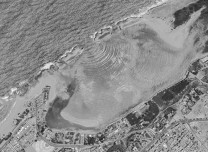
\includegraphics{images/sea-single-slit-diffraction.jpeg}
    \caption{Single slit diffraction.}
    \labfig{sea-single-slit-diffraction}
  \end{subfigure}
  \hfill
  \begin{subfigure}[b]{0.49\textwidth}
    \centering
    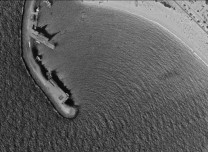
\includegraphics{images/sea-knife-edge-diffraction.jpeg}
    \caption{Knife-edge diffraction.}
    \labfig{sea-knife-edge-diffraction}
  \end{subfigure}
  \caption{Diffraction phenomena found in sea environments, Google Earth images.}
  \labfig{sea-diffraction}
\end{figure}

Diffraction is the mechanism that allows waves to bend around obstacles and propagate into \glspl{shadow region} where no \gls{line-of-sight} or reflected path exists. It is fundamentally explained by the \emph{Huygens--Fresnel principle}, which states that every point on a wavefront acts as a source of secondary spherical wavelets (see \reffig{huygens-principle}).

One of the most common examples of diffraction is called \emph{single slit diffraction}, where a wave passes through a narrow opening (i.e., small with respect to the \gls{wavelength}) and spreads out on the other side. This can be observed in \reffig{sea-single-slit-diffraction}. However, in the context of radio, especially outdoor propagation, a more common example of diffraction is \emph{knife-edge diffraction}, where a wave passes around a sharp obstacle, such as a mountain or a building. This can be observed in \reffig{sea-knife-edge-diffraction}.

\subsubsection{Single Knife-Edge Diffraction}

We first model diffraction of a plane wave over an absorbing plane or \emph{knife-edge}. The simple knife-edge diffraction model mathematically formulates Huygens' principle by combining contributions from an infinite number of secondary sources in the region above the edge.

\begin{figure}
  \centering
  \inputtikz{knife-edge-parameters}
  \caption{Knife-edge diffraction geometric parameters, reproduced from~\cite[Fig.~3.16]{Saunders2024}.}
  \labfig{knife-edge-parameters}
\end{figure}

The final result expresses the propagation loss, or reduction in field strength in decibels, in terms of a diffraction parameter $\nu$, which is defined as
\begin{equation}
  \nu = h'\sqrt{\frac{2\left(d_1' + d_2'\right)}{\lambda d_1' d_2'}},
\end{equation}
where $h'$ is the \emph{excess height} of the edge above the line from the transmitter to the receiver, $d_1'$ and $d_2'$ are the distances from the projection of the edge on this line to the transmitter and receiver, respectively, and $\lambda$ is the \gls{wavelength}, as illustrated in \reffig{knife-edge-parameters}.

The propagation loss is then given by
\begin{equation}
  L_{ke}(\nu) = -20 \log_{10}\left|\frac{\bsup{E}^d}{\bsup{E}^i}\right| = -20 \log_{10} |F(\nu)|,
\end{equation}
where $\bsup{E}^d$ is the diffracted field, $\bsup{E}^i$ is the incident field, and $F(\nu)$ is defined as
\begin{equation}\label{eq:transition-function-knife-edge}
  F(\nu) = \frac{1+j}{2} \int\limits_{\nu}^{\infty} \exp\left(-j \frac{\pi u^2}{2}\right) \,\mathrm{d}u,
\end{equation}

Alternatively, its magnitude can be expressed in terms of the Fresnel cosine and sine integrals, $C(\nu)$ and $S(\nu)$, which integrate the real and imaginary parts of the integrand from $0$ to $\nu$. To avoid complex values, we can write the squared magnitude of~\eqref{eq:transition-function-knife-edge} as
\begin{equation}
  |F(\nu)|^2 = \frac{1}{2} \left[ \left(\frac{1}{2} - C(\nu)\right)^2 + \left(\frac{1}{2} - S(\nu)\right)^2 \right],
\end{equation}
where
\begin{align}
  C(\nu) &= \int\limits_{0}^{\nu} \cos\left(\frac{\pi u^2}{2}\right) \,\mathrm{d}u, \\
  S(\nu) &= \int\limits_{0}^{\nu} \sin\left(\frac{\pi u^2}{2}\right) \,\mathrm{d}u.
\end{align}

While the Fresnel integrals lack closed-form analytical solutions in terms of elementary functions, they can be computed numerically or approximated using asymptotic expansions, which are available in most scientific computing libraries, such as the Cephes C library, on which many other libraries are built, such as SciPy's \texttt{scipy.special.fresnel} function.

\begin{figure}
  \centering
  \inputtikz{knife-edge-attenuation}
  \caption{Knife-edge diffraction loss $L_{ke}(\nu)$ as a function of the diffraction parameter $\nu$, reproduced from~\cite[Fig.~3.15]{Saunders2024}.}
  \labfig{knife-edge-attenuation}
\end{figure}

The knife-edge diffraction loss $L_{ke}$ is illustrated in \reffig{knife-edge-attenuation}. Notably, $L_{ke}(0) \approx \qty{6}{\decibel}$, which means that the power is reduced by a factor of $10^{0.6} \approx 4$ when the edge is situated exactly on the direct path between the transmitter and the receiver. For values $\nu > 1$, meaning for receivers well within the \gls{shadow region}, the attenuation increases significantly and can be approximated as
\begin{equation}
  L_{ke}(\nu) \approx -20 \log_{10} \frac{1}{\pi \nu \sqrt{2}} \approx -20 \log_{10} \frac{0.225}{\nu}.
\end{equation}

The parameter $\nu$ itself is tied to the geometry of the direct path relative to the edge, defined in \reffig{knife-edge-parameters} as
\begin{equation}
  \nu = h' \sqrt{\frac{2(d'_1 + d'_2)}{\lambda d'_1 d'_2}} = \alpha \sqrt{\frac{2 d'_1 d'_2}{\lambda(d'_1 + d'_2)}},
\end{equation}
where $h'$ is the excess height, and $d'_1$, $d'_2$ the distances from the source and receiver to the point of diffraction. For many practical cases where $d_1, d_2 \gg h$, this expression can be simplified in terms of distances measured along the ground
\begin{equation}
  \nu \approx h \sqrt{\frac{2(d_1 + d_2)}{\lambda d_1 d_2}} = \alpha \sqrt{\frac{2 d_1 d_2}{\lambda(d_1 + d_2)}},
\end{equation}
where $\alpha$ is the sum of the angles of elevation of the transmitter and receiver with respect to the knife-edge, $\beta$ and $\gamma$ in \reffig{knife-edge-parameters}, i.e.,
\begin{equation}
  \alpha = \beta + \gamma.
\end{equation}

An equivalent geometric interpretation uses Fresnel zones. Around the direct path, the first Fresnel-zone radius at a point located at distances $d_1$ and $d_2$ from transmitter and receiver is
\begin{equation}
  r_{F,1}=\sqrt{\frac{\lambda d_1 d_2}{d_1+d_2}}.
\end{equation}

\begin{figure*}
  \centering
  \inputtikz{fresnel-zones}
  \caption{First Fresnel zone around the direct path between two antennas.}
  \labfig{fresnel-zones}
\end{figure*}

See \reffig{fresnel-zones} for an illustration of the first Fresnel zone.

When an obstacle intrudes deeply into this first zone, diffraction loss rises rapidly. As a practical planning rule, preserving most of the first-zone clearance strongly reduces excess diffraction attenuation.

\subsubsection{Beyond Knife-Edge Diffraction}

While knife-edge diffraction provides valuable physical intuition and a tractable analytical solution based on Huygens' principle, it is fundamentally a simplified scalar model. It assumes the diffracting edge is part of a perfectly absorbing, semi-infinite screen and does not account for the actual structure, material properties, or finite extent of real obstacles. Moreover, it cannot handle oblique incidence, multiple edges, or wedges with arbitrary exterior angles.

In practical propagation scenarios, especially those encountered in urban environments, we frequently deal with complex geometries: building corners, rooftops, and terrain features that diffract electromagnetic waves in ways not captured by the knife-edge approximation. These situations require a more general, rigorous framework that preserves the full vector nature of electromagnetic fields, correctly handles polarization, and remains valid even in transition regions near shadow boundaries.

Such a framework is provided by the \emph{\gls{gtd}} and its mathematically uniform extension, the \emph{\gls{utd}}. These high-frequency asymptotic theories extend the ray concept to include diffracted rays emanating from edges, vertices, and other singular features. They provide dyadic diffraction coefficients analogous to Fresnel reflection coefficients, enabling precise prediction of field strength and polarization for arbitrary wedge geometries.

Because \gls{gtd} and \gls{utd} form the foundation of modern deterministic ray tracing for radio propagation, their detailed formulation, applicability conditions, and integration with geometrical optics are thoroughly presented in \refch{rt-fundamentals}, where we develop the complete mathematical machinery for ray-based channel modeling.

\subsection{Interaction with Metasurfaces}\labsec{metasurfaces}

\begin{marginfigure}
  \centering
  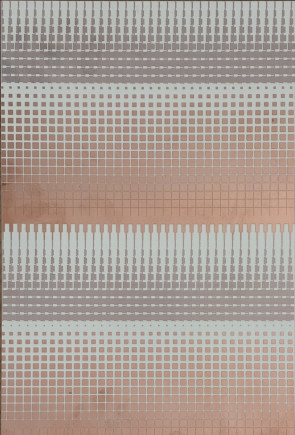
\includegraphics{images/metasurface.jpeg}
  \caption{Passive metasurface, kindly provided by Adam Abazi from the UCLouvain antenna group.}
  \labfig{metasurface}
\end{marginfigure}

Traditionally, the propagation of radio waves in wireless environments is dictated by the standard electromagnetic interactions discussed above: reflection, scattering, and diffraction. Standard specular reflection follows the conventional Snell's law (where the angle of incidence equals the angle of reflection), scattering disperses incident energy diffusely across multiple directions, and diffraction allows waves to bend around physical obstacles. In all of these standard interactions, the environment acts as a completely passive, unalterable medium that the communication system must adapt to.

A paradigm shift in this domain is the introduction of \emph{metasurfaces}. Metasurfaces are the two-dimensional, planar equivalents of metamaterials, composed of dense arrays of sub-\gls{wavelength} scattering elements (or unit cells) designed to engineer the electromagnetic wavefront, see \reffig{metasurface}. Unlike conventional surfaces, metasurfaces can generate a controllable, spatially varying phase, amplitude, or polarization shift across their aperture. By discretizing a continuous phase profile across its elements, a metasurface can manipulate waves in ways that natural materials cannot, such as by redirecting an incident wave toward an arbitrary, anomalous direction. This interaction is governed by the \emph{generalized Snell's law}~\sidecite{Yu2011} for reflection
\begin{equation}\label{eq:generalized-snell-reflection}
  \sin \theta_r - \sin \theta_i = \frac{\lambda _0}{2\pi} \frac{\mathrm{d}\Phi}{\mathrm{d}x},
\end{equation}
and for refraction
\begin{equation}\label{eq:generalized-snell-refraction}
  n_2 \sin \theta_t - n_1 \sin \theta_i = \frac{\lambda_0}{2\pi} \frac{\mathrm{d}\Phi}{\mathrm{d}x},
\end{equation}
where $n_1$ and $n_2$ are the refractive indices of the incident and transmitted media, $\theta_i$ is the angle of incidence, $\theta_r$ is the anomalous reflection angle, $\theta_t$ is the anomalous transmission angle, $\lambda_0$ is the \glshyph{free space} \gls{wavelength}, and $\tfrac{\mathrm{d}\Phi}{\mathrm{d}x}$ represents the phase gradient generated along the surface.

\begin{marginfigure}
  \centering
  \inputtikz{ris}
  \caption{A \glsxtrshort{ris}, inspired by~\cite[Fig.~1]{An2025}.}
  \labfig{ris}
\end{marginfigure}

A prominent and specific implementation of this technology in wireless communications is the \gls{ris}. A \gls{ris} is a dynamically tunable metasurface whose electromagnetic response can be electronically controlled (see \reffig{ris}). Built using printed conductive elements on a dielectric substrate and backed by a ground plane, a \gls{ris} integrates tunable components into each unit cell. This capability enables the creation of \enquote{smart radio environments} where the propagation channel itself becomes a programmable entity. Instead of merely adapting to random fading, systems can actively shape radio paths to bypass blockages, suppress interference, and enhance the overall link budget (see \reffig{ris-example}).

From a computational perspective, a \gls{ris} is usually the only kind of metasurface that we can easily and practically simulate using ray tracing. Because simulating the full-wave electromagnetic interactions of thousands of sub-\gls{wavelength} unit cells is computationally prohibitive, ray tracing engines generally avoid microscopic, element-level evaluations. Instead, we must rely on simplified macroscopic models that abstract the \gls{ris} into a continuous anomalous reflector or a grid of manageable tiles. These fundamental abstractions are crucial for efficient simulation, and we will present some of these simplified analytical models in \refch{rt-fundamentals}.

\begin{marginfigure}[-12\baselineskip]
  \centering
  \inputtikz{ris-example}
  \caption{Example scenario where a \glsxtrshort{ris} is used to redirect the signal towards the receiver, adapted from~\cite[Fig.~3]{Bjornson2022}.}
  \labfig{ris-example}
\end{marginfigure}

\section{Path Loss Models}\labsec{path-loss-models}

To evaluate the performance of a wireless communication system, one must predict the \emph{path loss}, which is the ratio of transmitted power to received power, usually expressed in decibels. While numerical methods offer extreme precision, several analytical models provide crucial insights into how propagation mechanisms dictate system range.

\subsection{Free-Space Path Loss}

In a completely empty void with only a \gls{line-of-sight} link, the received power $P_r$ is related to the transmitted power $P_t$ by the (contemporary) \emph{Friis transmission equation}~\sidecite{Friis1946}
\begin{equation}
  \frac{P_r}{P_t} = G_t G_r \left(\frac{\lambda}{4\pi d}\right)^2,
\end{equation}
where $G_t$ and $G_r$ are the peak gains of the transmitting and receiving antennas, respectively, and $d$ is the distance between the two antennas.

Because the term $\left(\tfrac{\lambda}{4\pi d}\right)^2$ dictates the power decay, the \glshyph{free space} path loss increases quadratically with distance. Consequently, the signal drops by \qty{20}{\decibel} per decade (i.e., every time the distance increases tenfold). This represents the theoretical minimum loss for point-to-point propagation when multipath effects are neglected.

\subsection{The Two-Ray Ground Reflection Model}

\begin{figure}
  \inputtikz{two-ray-model}
  \caption{The two-ray ground reflection model parameters.}
  \labfig{two_ray_model}
\end{figure}

Environments on Earth are rarely true \gls{line-of-sight} \gls{free space} scenarios; most of the time, the ground at least plays a role in reflecting waves. The interaction between a direct path and a ground-reflected path (see \reffig{two_ray_model}) illustrates the concept of multipath interference.

In the two-ray ground reflection model, the received signal consists of two components: the \gls{line-of-sight} ray and the ray reflected by the ground. The total received electric field is the sum of these two contributions. Using the parameters defined in \reffig{two_ray_model}, where $d'$ is the length of the direct path and $d_1 + d_2$ is the length of the reflected path, the received power $P_r$ can be expressed as an extension of the Friis transmission equation
\begin{equation}
  P_r = P_t G_t G_r \left( \frac{\lambda}{4\pi} \right)^2 \left| \frac{e^{-jk d'}}{d'} + R \frac{e^{-jk (d_1 + d_2)}}{d_1 + d_2} \right|^2,
\end{equation}
where $R$ is the ground reflection coefficient, which depends, as we have seen in \refsec{reflection-and-transmission}, on the electromagnetic properties of the ground, the polarization, and the angle of incidence $\theta=\tfrac{\pi}{2}-\alpha$.

For most practical scenarios, especially in macrocellular communications, the horizontal distance $d$ separating the transmitter and receiver is much larger than their respective heights $h_t$ and $h_r$ ($d \gg h_t, h_r$). Under this condition, the lengths of the two paths can be approximated using a Taylor series expansion
\begin{align}
  d' &= \sqrt{d^2 + (h_t - h_r)^2} \approx d + \frac{(h_t - h_r)^2}{2d}, \\
  d_1 + d_2 &= \sqrt{d^2 + (h_t + h_r)^2} \approx d + \frac{(h_t + h_r)^2}{2d}.
\end{align}
The path difference $\Delta d \eqdef d_1 + d_2 - d'$ then simplifies to
\begin{equation}
  \Delta d \approx \frac{(h_t + h_r)^2 - (h_t - h_r)^2}{2d} = \frac{2 h_t h_r}{d}.
\end{equation}
This path difference translates to a phase difference $\Delta \phi$ between the two rays given by
\begin{equation}
  \Delta \phi = k \Delta d = \frac{2\pi}{\lambda} \frac{2 h_t h_r}{d} = \frac{4\pi h_t h_r}{\lambda d}.
\end{equation}

At large distances, the incidence angle approaches a grazing angle ($\alpha \to 0$, $\theta \to \tfrac{\pi}{2}$). In this grazing incidence case, the reflection coefficient for both polarizations approaches $-1$ (i.e., $R \approx -1$). Furthermore, since $d \gg h_t, h_r$, we can approximate the denominators in the received power equation as $d' \approx d_1 + d_2 \approx d$. The power equation then becomes
\begin{equation}
  P_r \approx P_t G_t G_r \left( \frac{\lambda}{4\pi d} \right)^2 \left| 1 + R e^{-j\Delta \phi} \right|^2.
\end{equation}

Substituting $R \approx -1$ into this expression yields $1 + R e^{-j\Delta \phi} \approx 1 - e^{-j\Delta \phi}$, which indicates that the reflected wave arrives with an inverted phase relative to the direct wave, causing destructive interference. For very small phase differences $\Delta \phi \ll 1$ (which holds true at large distances), we can use the small-angle approximation $e^{-j\Delta \phi} \approx 1 - j\Delta \phi$. The magnitude squared of the interference term simplifies to
\begin{equation}
  \left| 1 - (1 - j\Delta \phi) \right|^2 = |j\Delta \phi|^2 = (\Delta \phi)^2 = \left( \frac{4\pi h_t h_r}{\lambda d} \right)^2.
\end{equation}

Substituting this back into the power equation yields the simplified two-ray path loss model for large distances
\begin{equation}\label{eq:two-ray-approx}
  P_r \approx P_t G_t G_r \left( \frac{\lambda}{4\pi d} \right)^2 \left( \frac{4\pi h_t h_r}{\lambda d} \right)^2 = P_t G_t G_r \frac{h_t^2 h_r^2}{d^4}.
\end{equation}

\begin{figure*}
  \centering
  \inputtikz{two-ray-power}
  \caption{Received power gain for the two-ray ground reflection model as a function of the distance ($h_t = \qty{10}{\meter}$, $h_r = \qty{1.5}{\meter}$, $f = \qty{2.4}{\giga\hertz}$), showing the direct path, reflected path, and total received power for both parallel ($\parallel$) and perpendicular ($\perp$) polarizations. The electromagnetic properties of the ground are approximated as \enquote{medium dry ground} from ITU-R Recommendation P.2040~\cite[Tab.~3]{ITU-R-P.2040}.}
  \labfig{two-ray-power}
\end{figure*}

This fundamental result demonstrates that at large distances, destructive multipath interference changes the path loss distance exponent from $2$ (in \gls{free space}) to $4$ (see \reffig{two-ray-power}). This means the power falls off at a rapid \qty{40}{\decibel} per decade, and is notably independent of the frequency. The two-ray model serves as a baseline demonstrating that environmental interactions severely and predictably impact signal decay in terrestrial environments, particularly highlighting the effect of the ground.

In practice, the transition toward this asymptotic $d^{-4}$ regime can be approximated to start at a breakpoint distance, $d_{\mathrm{bp}}$, defined as
\begin{equation}
  d_{\mathrm{bp}} \approx \frac{4 h_t h_r}{\lambda},
\end{equation}
which corresponds to the range where the first Fresnel zone starts to be significantly clipped by the ground-reflected geometry. For $d \ll d_{\mathrm{bp}}$, the behavior is closer to \glshyph{free space} scaling; for $d \gg d_{\mathrm{bp}}$, the asymptotic two-ray law becomes a good approximation.

\subsection{The Link Budget}

The complete assessment of all gains and losses from transmitter to receiver forms the \emph{link budget}. For this, we identify two types of losses: antenna losses and propagation---or path---losses.

For the antennas, we express their gain with respect to an isotropic antenna. The \gls{eirp} is given by
\begin{equation}
  \text{\gls{eirp}} = \frac{P_t G_t}{L_t} = P_{t,\text{iso}},
\end{equation}
where $L_t$ is the loss in the transmitting antenna system and $P_{t,\text{iso}}$ is the effective isotropic transmitted power.

A similar value can be obtained for the receiver
\begin{equation}
  P_{r,\text{iso}} = \frac{P_r G_r}{L_r},
\end{equation}
where $L_r$ is the loss in the receiving antenna system and $P_{r,\text{iso}}$ is the effective isotropic received power.

Knowing the effective isotropic transmitted and received power, it is possible to determine the path loss
\begin{equation}
  L = \frac{P_{t,\text{iso}}}{P_{r,\text{iso}}} = \frac{P_t G_t G_r}{P_r L_t L_r}.
\end{equation}

However, it is rarely desirable to determine the path loss through actual measurements, as it requires---usually expensive---equipment, can be time-consuming, and provides values that are not easily generalizable to other environments or system configurations. As a result, path loss models are crucial for predicting how the signal strength varies in a given environment.

\section{Conclusion}

This chapter has established the physical \enquote{ground truth} of radio propagation. We have seen how Maxwell's equations give rise to waves that propagate, reflect, and transmit. We also introduced the antennas that launch these waves. Note that throughout these analytical models, the propagation medium (air) is almost universally approximated as an ideal \gls{free space} ($\epsilon_r \approx 1, \sigma \approx 0$), with all significant interactions isolated to the boundaries of solid objects.

To determine the signal strength at a receiver in a complex environment like a city, one might consider solving Maxwell's equations numerically for every point in space and time. Full-wave electromagnetic solvers based on methods like \gls{fdtd}, \gls{fem}, or \gls{mom} offer extreme precision. However, because they require meshing the entire volume or surfaces at sub-\gls{wavelength} resolutions, they become computationally intractable for environments larger than a few cubic meters, especially at high frequencies.

Conversely, the simple analytical path loss models discussed in \refsec{path-loss-models} scale effortlessly but are far too simplistic to capture the severe multipath fading induced by hundreds of building facades and terrain variations.

To simulate radio propagation efficiently and accurately at the urban scale, we need a method that simplifies wave interactions into geometric paths, avoiding the need to discretize empty space. \Glsxtrfull{go} and \gls{utd} provide this perfect middle ground. As briefly introduced both by the knife-edge diffraction and the two-ray models, we will rely on ray tracing to simulate radio propagation in complex environments. In the next chapter, we will introduce the \emph{high-frequency approximation}, which allows us to transition from the wave domain to the ray domain, forming the mathematical basis of the ray tracing algorithms we aim to construct in \arefpart{building}.
